\begin{figure}
  \centering
    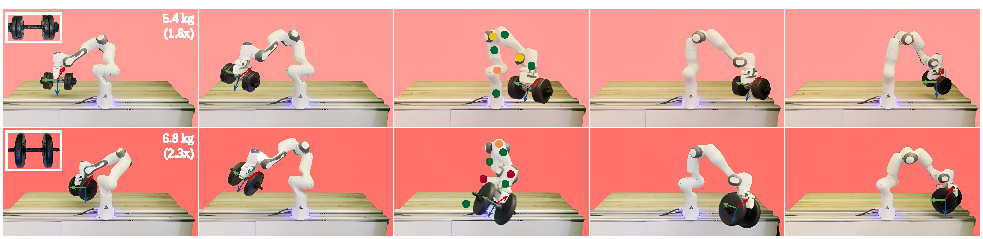
\includegraphics[width=\columnwidth]{graphics/vignew.pdf}
  \caption{Two qualitative motions of the robot carrying super-nominal payloads of \textcolor{pink}{$5.4$kg ($1.8\times$ nominal capacity)} and \textcolor{pastelred}{$6.8$kg ($2.3\times$ nominal capacity)} are shown. Colored dots indicate joint torques as a percentage of joint limits: \textcolor{green}{$0-20\%$}, \textcolor{midgreen}{$20-40\%$}, \textcolor{mid}{$40-60\%$}, \textcolor{midred}{$60-80\%$}, \textcolor{red}{$80-100\%$}. Joints 1, 3, and 5 exhibit higher torques, with joint 1 bearing the structural load of the arm and joints 3 and 5 positioning and orienting the payload.\vspace{-0.2in}}\label{fig:vignette}
\end{figure}